\documentclass[11pt,a4paper]{article}

%% ── packages ─────────────────────────────────────────────────────────────────
\usepackage[T1]{fontenc}
\usepackage[utf8]{inputenc}
\usepackage{helvet}
\renewcommand{\familydefault}{\sfdefault}
\usepackage[margin=20mm,top=22mm,bottom=24mm]{geometry}
\usepackage{microtype}
\usepackage{xcolor}
\usepackage{tikz}
\usetikzlibrary{shapes.geometric,arrows.meta,positioning,calc,decorations.pathmorphing,backgrounds,fit}
\usepackage[most]{tcolorbox}
\usepackage{listings}
\usepackage{fancyhdr}
\usepackage{titlesec}
\usepackage{mdframed}
\usepackage{tabularx}
\usepackage{booktabs}
\usepackage{array}
\usepackage{enumitem}
\usepackage{multicol}
\usepackage{environ}
\usepackage{etoolbox}
\usepackage{parskip}
\usepackage{amssymb}
\usepackage{hyperref}
\setlength{\headheight}{22pt}

%% ── palette ──────────────────────────────────────────────────────────────────
\definecolor{Ink}        {HTML}{1A1A2E}
\definecolor{SlateDeep}  {HTML}{16213E}
\definecolor{Slate}      {HTML}{0F3460}
\definecolor{Teal}       {HTML}{0F6E56}
\definecolor{TealLight}  {HTML}{E1F5EE}
\definecolor{TealMid}    {HTML}{1D9E75}
\definecolor{Purple}     {HTML}{534AB7}
\definecolor{PurpleLight}{HTML}{EEEDFE}
\definecolor{PurpleMid}  {HTML}{7F77DD}
\definecolor{Amber}      {HTML}{BA7517}
\definecolor{AmberLight} {HTML}{FAEEDA}
\definecolor{AmberMid}   {HTML}{EF9F27}
\definecolor{Coral}      {HTML}{993C1D}
\definecolor{CoralLight} {HTML}{FAECE7}
\definecolor{CoralMid}   {HTML}{D85A30}
\definecolor{Blue}       {HTML}{185FA5}
\definecolor{BlueLight}  {HTML}{E6F1FB}
\definecolor{BlueMid}    {HTML}{378ADD}
\definecolor{GrayLight}  {HTML}{F1EFE8}
\definecolor{GrayMid}    {HTML}{888780}
\definecolor{GrayBorder} {HTML}{D3D1C7}
\definecolor{Red}        {HTML}{A32D2D}
\definecolor{RedLight}   {HTML}{FCEBEB}
\definecolor{Green}      {HTML}{3B6D11}
\definecolor{GreenLight} {HTML}{EAF3DE}

%% ── hyperref ─────────────────────────────────────────────────────────────────
\hypersetup{colorlinks=true,linkcolor=Purple,urlcolor=Blue,citecolor=Teal,
            pdftitle={VSEPR-SIM Engineering Scope: Output Stack, .dynx Pipeline, .X Bundle},
            pdfauthor={VSEPR-SIM Engineering}}

%% ── listings ─────────────────────────────────────────────────────────────────
\lstdefinestyle{vsim}{
  basicstyle=\ttfamily\footnotesize\color{Ink},
  backgroundcolor=\color{GrayLight},
  frame=none,
  breaklines=true,
  breakatwhitespace=true,
  keepspaces=true,
  columns=fullflexible,
  showstringspaces=false,
  tabsize=2,
  commentstyle=\color{GrayMid}\itshape,
  keywordstyle=\color{Purple}\bfseries,
  stringstyle=\color{Teal},
  rulecolor=\color{GrayBorder},
  xleftmargin=6pt,
  xrightmargin=6pt,
  aboveskip=4pt,
  belowskip=4pt,
}
\lstset{style=vsim}

%% ── tcolorbox styles ─────────────────────────────────────────────────────────
\tcbuselibrary{breakable,skins,listings}

\newtcolorbox{wobox}[3][]{
  enhanced,breakable,
  colback=#2!8!white, colframe=#2, colbacktitle=#2, coltitle=white,
  fonttitle=\bfseries\large, title={#3},
  arc=6pt, boxrule=0.8pt, left=8pt, right=8pt, top=6pt, bottom=6pt,
  titlerule=0pt,
  attach boxed title to top left={yshift=-2mm,xshift=6mm},
  boxed title style={arc=4pt,boxrule=0pt,colback=#2}, #1
}

\newtcolorbox{purposebox}[2][]{
  enhanced,breakable,
  colback=#2!6!white, colframe=#2!40!white,
  leftrule=4pt, toprule=0.3pt, bottomrule=0.3pt, rightrule=0.3pt,
  arc=3pt, left=8pt, right=8pt, top=5pt, bottom=5pt, #1
}

\newtcolorbox{notebox}[2][]{
  enhanced,breakable,
  colback=#2!8!white, colframe=#2!50!white,
  leftrule=3pt, toprule=0.3pt, bottomrule=0.3pt, rightrule=0.3pt,
  arc=3pt, left=7pt, right=7pt, top=4pt, bottom=4pt,
  fontupper=\footnotesize, #1
}

\newtcolorbox{codebox}[1][]{
  enhanced,breakable,
  colback=GrayLight, colframe=GrayBorder,
  arc=4pt, boxrule=0.5pt, left=6pt, right=6pt, top=4pt, bottom=4pt,
  fontupper=\ttfamily\footnotesize\color{Ink}, #1
}

\newcommand{\chip}[2]{%
  \colorbox{#1}{\color{white}\bfseries\tiny\MakeUppercase{#2}}}
\newcommand{\badge}[2]{%
  \fcolorbox{#1!40!white}{#1!10!white}{\color{#1!80!black}\bfseries\tiny\MakeUppercase{#2}}}
\newcommand{\pipenode}[1]{%
  \colorbox{GrayLight}{\strut\,\footnotesize#1\,}}
\newcommand{\pipearrow}{\;\textcolor{GrayMid}{$\to$}\;}
\newcommand{\chk}{\textcolor{Teal}{\textbf{\checkmark}}\;}
\newcommand{\wo}[1]{\texttt{\color{Slate}#1}}

%% ── section rules ────────────────────────────────────────────────────────────
\titleformat{\section}{\large\bfseries\color{Ink}}{}{0pt}{}[{\color{GrayBorder}\titlerule[0.5pt]}]
\titlespacing{\section}{0pt}{14pt}{6pt}
\titleformat{\subsection}{\normalsize\bfseries\color{Slate}}{}{0pt}{}
\titlespacing{\subsection}{0pt}{10pt}{4pt}

%% ── header / footer ──────────────────────────────────────────────────────────
\pagestyle{fancy}
\fancyhf{}
\fancyhead[L]{\small\color{GrayMid}\textbf{VSEPR-SIM} \textbar\ Engineering Scope Reference}
\fancyhead[R]{\small\color{GrayMid}Output Stack \textbullet\ .dynx \textbullet\ .X Bundle \textbullet\ v5.1.x}
\fancyfoot[C]{\small\color{GrayMid}\thepage}
\renewcommand{\headrulewidth}{0.4pt}
\renewcommand{\headrule}{\hbox to\headwidth{\color{GrayBorder}\leaders\hrule height \headrulewidth\hfill}}

%% ── document ─────────────────────────────────────────────────────────────────
\begin{document}

%% ── COVER ────────────────────────────────────────────────────────────────────
\thispagestyle{empty}
\begin{tikzpicture}[remember picture,overlay]
  \fill[SlateDeep] (current page.north west) rectangle ([yshift=-88mm]current page.north east);
  \fill[Teal]      ([yshift=-88mm]current page.north west) rectangle ([yshift=-92mm]current page.north east);
  \fill[Purple]    ([yshift=-92mm]current page.north west) rectangle ([yshift=-94mm]current page.north east);
\end{tikzpicture}

\vspace*{22mm}
{\color{white}\fontsize{28}{34}\selectfont\bfseries VSEPR-SIM\par}
\vspace{3mm}
{\color{TealMid}\fontsize{16}{20}\selectfont Engineering Scope Reference\par}
\vspace{5mm}
{\color{white!70!SlateDeep}\large Output Stack \textbullet\ .dynx Pipeline \textbullet\ .X Bundle \textbullet\ v5.1.x\par}
\vspace{3mm}
{\color{white!50!SlateDeep}\normalsize
\wo{WO-OUTPUT-P2} \textbullet\ \wo{WO-72A} \textbullet\ \wo{WO-72B} \textbullet\ \wo{WO-VSIM-CTL} \textbullet\ \wo{WO-67-B}\par}
\vspace{36mm}

\begin{tikzpicture}
  \node[fill=TealLight,draw=Teal,line width=0.8pt,rounded corners=6pt,
        inner sep=10pt,text width=\linewidth-24pt]{%
    \color{Ink}\small
    \textbf{Document scope.}\enspace
    This reference covers the implemented output and viewer pipeline as it exists in the
    \texttt{v5.0.0-main} / \texttt{v5.1.x} codebase: the demo artifact stack
    (\wo{WO-OUTPUT-P2}), the \texttt{.X} suite bundle format (\wo{WO-72A}), the
    \texttt{.dynx} rich-frame emitter pipeline (\wo{WO-72B}), the modernised VSIM
    control pipeline (\wo{WO-VSIM-CTL}), and the viewer file-type data contract
    (\wo{WO-67-B}).
    All sections describe code that is \emph{built, tested, and passing}
    --- not planned features.
  };
\end{tikzpicture}

\vfill
{\color{GrayMid}\footnotesize VSEPR-SIM Engineering \textbar\ Internal Use \textbar\ v5.1.x}
\newpage

%% ── TABLE OF CONTENTS ────────────────────────────────────────────────────────
\tableofcontents
\newpage

%% ════════════════════════════════════════════════════════════════════════════
\section{\texorpdfstring{\chip{Teal}{WO-OUTPUT-P2}}{WO-OUTPUT-P2}\enspace Output System Expansion --- Phase 2: Demo Stack}
%% ════════════════════════════════════════════════════════════════════════════

\badge{Teal}{COMPLETE}\quad\badge{Blue}{Schema}\quad\badge{Amber}{IO Layer}

\subsection*{Purpose}
\begin{purposebox}{Teal}
Produce condensed, self-contained molecular demonstration artifacts from batch and single
simulation runs.  A ``demo artifact'' is a lightweight snapshot of a run --- not a replay
of the full trajectory --- suitable for embedding in reports, CI pipelines, and interactive
review.  The stack adds three new layers on top of the existing \texttt{.dynx} writer:
a schema section, a frame sampler, and a bundle writer.
\end{purposebox}

\subsection*{Schema: \texttt{[export.demo]} --- \texttt{ExportDemoSection}}

Declared in \texttt{include/vsim/vsim\_document.hpp}.  All fields have safe defaults;
the section is off by default (\texttt{enabled = false}).

\begin{lstlisting}
struct ExportDemoSection {
    bool        enabled           = false;   // master switch
    int         demo_frames       = 10;      // max frames to include
    std::string strategy          = "uniform";
    // "first" | "last" | "uniform" | "event_gated"
    bool        write_demo_dynx   = true;    // emit <case>.demo.dynx
    bool        write_demo_bundle = true;    // emit <case>.demo.X
    bool        include_source    = true;    // embed .vsim in bundle
    bool        include_manifest  = true;    // embed demo_manifest.json
    std::string bundle_name;                 // override name (auto if empty)
};
\end{lstlisting}

VSIM config block:

\begin{lstlisting}
[export.demo]
enabled        = true
demo_frames    = 12
strategy       = "uniform"       # first | last | uniform | event_gated
write_demo_dynx   = true
write_demo_bundle = true
include_source    = true
include_manifest  = true
\end{lstlisting}

\subsection*{DemoFrameSampler --- \texttt{include/vsim/io/demo\_frame\_sampler.hpp}}

Selects frames from a \texttt{DynxReader} archive according to \texttt{ExportDemoSection::strategy}:

\begin{center}
\begin{tabularx}{\linewidth}{@{}lX@{}}
\toprule
\textbf{Strategy} & \textbf{Behaviour} \\
\midrule
\texttt{first}       & Frames $0 \ldots \min(\textit{demo\_frames}-1, N-1)$ \\
\texttt{last}        & Last \textit{demo\_frames} frames from the archive \\
\texttt{uniform}     & Evenly spaced indices across the full archive (default) \\
\texttt{event\_gated} & Only frames containing at least one \texttt{EVENT} packet \\
\bottomrule
\end{tabularx}
\end{center}

The sampler operates on already-written \texttt{.dynx} archives; it does not buffer frames in memory.

\subsection*{DemoBundleWriter --- \texttt{include/vsim/io/demo\_bundle\_writer.hpp}}

Consumes sampled frames from \texttt{DemoFrameSampler} and emits two artifacts:

\begin{enumerate}[leftmargin=*,itemsep=2pt]
  \item \textbf{\texttt{<case>.demo.dynx}} --- a condensed \texttt{.dynx} archive containing only the sampled frames, in standard Dynx v1 format.  Readable by any \texttt{DynxReader}.
  \item \textbf{\texttt{<case>.demo.X}} --- a self-contained \texttt{.X} bundle embedding the \texttt{.demo.dynx} file, the originating \texttt{.vsim} script, and a \texttt{demo\_manifest.json} provenance record.
\end{enumerate}

\subsection*{Batch aggregator hook}

\texttt{run\_demo\_artifacts()} is called by the batch post-run hook after each run completes.
It resolves the run's \texttt{.dynx} path, instantiates a \texttt{DemoFrameSampler} and
\texttt{DemoBundleWriter}, and writes the demo artifacts into the run output directory.
The call is gated on \texttt{ExportDemoSection::enabled} and is a no-op when the section is absent.

\subsection*{Output files}
\begin{codebox}
<run_dir>/<case>.demo.dynx         (condensed Dynx v1 archive)
<run_dir>/<case>.demo.X            (self-contained bundle)
<run_dir>/demo_manifest.json       (provenance: source, strategy, frame indices)
\end{codebox}

\subsection*{Test coverage}

\begin{center}
\begin{tabularx}{\linewidth}{@{}lllX@{}}
\toprule
\textbf{Group} & \textbf{Name} & \textbf{Assertions} & \textbf{Coverage} \\
\midrule
73 & \texttt{ExportDemoSectionGroup73} & 25 & Schema defaults, parser round-trip, all strategy strings \\
74 & \texttt{DemoFrameSamplerGroup74}  & 21 & Sampler strategies, reduced archive generation, edge cases \\
75 & \texttt{DemoBundleWriterGroup75}  & 19 & Bundle round-trip, manifest embedding, source inclusion \\
\bottomrule
\end{tabularx}
\end{center}

\begin{notebox}{Teal}
\textbf{Build gate:} All three groups pass.
Full \texttt{ninja} build exits 0 with zero regressions.
\end{notebox}

\newpage
%% ════════════════════════════════════════════════════════════════════════════
\section{\texorpdfstring{\chip{Purple}{WO-72A}}{WO-72A}\enspace .X Bundle Format}
\label{sec:xbundle}
%% ════════════════════════════════════════════════════════════════════════════

\badge{Purple}{COMPLETE}\quad\badge{Blue}{Format}

\subsection*{Purpose}
\begin{purposebox}{Purple}
The \texttt{.X} format is a bundled suite-execution container.  It packs one or more
\texttt{.vsim} scripts (or inline script text), optional assets, dependency ordering,
and expected output declarations into a single text file that the \texttt{vsepr} CLI
can execute as an ordered unit.  It is also a reproducibility artifact: it carries the
run seed, version tag, and a SHA-1 hash of each included script so that replaying the
bundle produces identical outputs given the same binary.
\end{purposebox}

\subsection*{Role separation}

\begin{center}
\begin{tabularx}{\linewidth}{@{}lX@{}}
\toprule
\textbf{Format} & \textbf{Role} \\
\midrule
\texttt{.vsim}      & Human-authored source script \\
\texttt{.xyz} / \texttt{.xyzFull} & Scientific state / replay truth \\
\texttt{.dynx}      & Live visual / session archive (post-compiled) \\
\texttt{.X}         & Bundled suite-execution container \\
\bottomrule
\end{tabularx}
\end{center}

\subsection*{Data model --- \texttt{include/vsim/bundle/x\_bundle.hpp}}

\begin{lstlisting}
// Slot kinds
enum class XBundleSlotKind : uint8_t {
    Script, InlineScript, PyKernel, ValidationCheck, Benchmark
};

struct XBundleSlot {
    std::string id;              // unique slot id within bundle
    std::string label;           // human label, e.g. "ANN-01 identity gate"
    XBundleSlotKind kind;
    std::string script_path;     // for Script / PyKernel kinds
    std::string inline_text;     // for InlineScript kind
    std::vector<XBundleOverride> overrides;
    std::vector<std::string>     depends_on;  // ordered dependency ids
    std::vector<XBundleOutput>   expected_outputs;
    double max_wall_s  = 0.0;    // 0 = no limit
    bool   allow_failure = false;
    std::string script_hash_sha1;  // verified before execution
};

struct XBundleManifest {
    std::string  bundle_id;      // script-defined; no hardcoded defaults
    std::string  version;
    std::string  purpose;
    std::string  author;
    std::string  created_utc;
    uint64_t     run_seed = 0;
    std::string  vsim_version;
    std::string  git_ref;
    std::vector<XBundleSlot> slots;
    std::string  summary_md_path;
    std::string  events_jsonl_path;
    std::string  bench_tsv_path;
    bool   abort_on_first_failure = false;
    double global_wall_limit_s    = 0.0;
};
\end{lstlisting}

\subsection*{Slot outcomes}

\begin{center}
\begin{tabularx}{\linewidth}{@{}lX@{}}
\toprule
\textbf{Outcome} & \textbf{Meaning} \\
\midrule
\texttt{Pending}  & Not yet started \\
\texttt{Running}  & Currently executing \\
\texttt{Passed}   & Completed; all expected outputs present and valid \\
\texttt{Failed}   & Slot or output assertion failed \\
\texttt{Skipped}  & A dependency failed; slot was bypassed \\
\bottomrule
\end{tabularx}
\end{center}

\subsection*{Typical use cases}

\begin{multicols}{2}
\begin{itemize}[leftmargin=*,itemsep=2pt]
  \item[\chk] Annihilation test ladders (ANN-01..10)
  \item[\chk] Formation sweeps with multiple seeds
  \item[\chk] Benchmark suites run by CI
  \item[\chk] Multi-step validation chains
  \item[\chk] Demo bundle embedding (WO-OUTPUT-P2)
  \item[\chk] Post-compiled \texttt{.dynx} + \texttt{.vsim} pairs
\end{itemize}
\end{multicols}

\subsection*{Annihilation test ladder factory}

The header provides \texttt{make\_annihilation\_test\_bundle(seed, script\_dir)} which
constructs the canonical ANN-01 through ANN-10 slot sequence with correct dependency
ordering.  Slot ANN-04 depends on ANN-02 \emph{and} ANN-03 (both gates must pass before
product records are created).

\subsection*{Test coverage}

Group 70 (\texttt{XBundleSmokeGroup70}) --- 10 assertions covering manifest construction,
slot lookup, dependency ordering, and outcome classification.
\textbf{144/144 tests pass. Zero regressions.}

\newpage
%% ════════════════════════════════════════════════════════════════════════════
\section{\texorpdfstring{\chip{Amber}{WO-72B}}{WO-72B}\enspace .dynx Pipeline Emitter}
\label{sec:dynx}
%% ════════════════════════════════════════════════════════════════════════════

\badge{Amber}{COMPLETE}\quad\badge{Blue}{IO Layer}\quad\badge{Teal}{Archive + Live}

\subsection*{Purpose}
\begin{purposebox}{Amber}
The \texttt{.dynx} format is a post-compiled dynamic session archive.  WO-72B adds the
\emph{emitter pipeline}: a post-step hook that consumes rich simulation state each FIRE
step and simultaneously writes a persistent \texttt{.dynx} archive \emph{and} pushes
the latest frame into a thread-safe live cache polled by the viewer.
\end{purposebox}

\subsection*{Dynx v1 wire format}

\begin{lstlisting}
#dynx v1
#source <path>
#source_hash <sha256-hex | "none">
#kernel_version <string>
#frame_count <N>
#frame_interval <dt_fs>
#particle_count <N>
#timestamp <ISO-8601>
FRAME <index> <time_fs>
<N> <symbol> <x> <y> <z> [<vx> <vy> <vz>] [<energy>]
FORCE      <idx> <fx> <fy> <fz>               (optional)
BOND_FORCE <i> <j> <bfx> <bfy> <bfz>         (optional)
FIELD      <label> <fx> <fy> <fz>             (optional)
EVENT      <kind> <event_id> <source> <value> (optional)
RENDER     <idx> <r> <g> <b> <tag> <visible>  (optional)
CAMERA     <label> <x> <y> <z> <pitch> <yaw> <zoom> (optional)
END_FRAME
...
#END_DYNX
\end{lstlisting}

\begin{notebox}{Blue}
Optional lines (\texttt{FORCE}, \texttt{BOND\_FORCE}, \texttt{FIELD}, \texttt{EVENT},
\texttt{RENDER}, \texttt{CAMERA}) are forward-compatible: unknown prefixes are silently
skipped by v1 readers.  Velocities and per-particle energy are also optional.
\end{notebox}

\subsection*{Rich-frame data structs --- \texttt{include/vsim/io/dynx\_writer.hpp}}

\begin{lstlisting}
struct DynxForceState  { int idx; std::array<double,3> force; };
struct DynxBondForce   { int i, j; std::array<double,3> force; };
struct DynxFieldVector { std::string label; std::array<double,3> vec; };
struct DynxEventPacket {
    std::string kind;    // "reaction" | "checkpoint" | "phase_transition"
    uint64_t    event_id = 0;
    std::string source;  // source_formula from KernelEvent
    double      value    = 0.0;
};
struct DynxRenderMeta  {
    int particle_idx;
    uint8_t r, g, b;    // RGB colour override
    std::string tag;
    bool visible = true;
};
struct DynxCameraState {
    std::string label;   // "default" | "close_up" | ...
    // x, y, z, pitch, yaw, zoom
};
struct DynxRichFrame {
    DynxFrame                    base;
    std::vector<DynxForceState>  forces;
    std::vector<DynxBondForce>   bond_forces;
    std::vector<DynxFieldVector> field_vectors;
    std::vector<DynxEventPacket> events;
    std::vector<DynxRenderMeta>  render_meta;
    std::vector<DynxCameraState> cameras;
};
\end{lstlisting}

\subsection*{Emitter architecture}

\medskip\noindent
\pipenode{FIRE step}
\pipearrow\pipenode{\texttt{DynxEmitter::emit\_step()}}
\pipearrow\pipenode{\texttt{DynxWriter::write\_rich\_frame()}}
\par\noindent\hspace{6em}\pipearrow\pipenode{\texttt{DynxLiveCache::push()}}
\medskip

\begin{description}[leftmargin=*,itemsep=3pt]
  \item[\texttt{DynxWriter}] Streams rich frames to a \texttt{.dynx} file.
    Backward-compatible with v1 baseline readers.
  \item[\texttt{DynxEmitter}] Post-step hook.  Calls
    \texttt{KernelEventLog::instance().filter\_by\_frame(fid, fid)} to harvest
    matching events automatically, then calls \texttt{write\_rich\_frame()}.
    Pushes a copy of the frame to \texttt{DynxLiveCache}.
  \item[\texttt{DynxLiveCache}] Mutex-guarded single-slot cache.  \texttt{push()} replaces
    any existing slot.  \texttt{poll()} returns the frame \emph{and clears the slot}.
    The viewer calls \texttt{poll()} each render tick; no frame is stale.
\end{description}

\begin{notebox}{Amber}
\textbf{Live cache without archive.}
\texttt{emit\_step()} without a prior \texttt{open()} call still pushes to
\texttt{DynxLiveCache} and returns \texttt{true}.  No archive file is required
for the live viewer path.
\end{notebox}

\subsection*{KernelEvent harvesting}

\texttt{DynxEmitter::emit\_step()} calls:

\begin{lstlisting}
KernelEventLog::instance().filter_by_frame(frame_id, frame_id)
\end{lstlisting}

Events matching the current frame are automatically appended as \texttt{EVENT} packets
in the rich frame, in addition to any caller-supplied events in \texttt{DynxEmitContext}.

\subsection*{Test coverage}

Group 71 (\texttt{DynxEmitterGroup71}) --- 15 test cases, 29 assertions (71-A through 71-O):
live cache push/poll/clear, rich-frame write/read round-trip, event harvesting,
archive-open gating, and full emitter pipeline.
\textbf{145/145 tests pass.  Zero regressions.}

\newpage
%% ════════════════════════════════════════════════════════════════════════════
\section{\texorpdfstring{\chip{Blue}{WO-67-B}}{WO-67-B}\enspace Viewer File-Type Data Contract}
\label{sec:viewcontract}
%% ════════════════════════════════════════════════════════════════════════════

\badge{Blue}{COMPLETE}\quad\badge{Slate}{Contract Layer}

\subsection*{Purpose}
\begin{purposebox}{Blue}
The viewer is a \emph{dumb renderer}: it reads decoded state from a canonical
\texttt{ViewFrame} and renders it.  It never reads simulation internals directly
and never mutates physical state.  WO-67-B defines the authoritative contract between
each supported file type and the \texttt{ViewFrame}, specifying what each loader
\emph{must} and \emph{may} contribute.
\end{purposebox}

\subsection*{File-type contract table}

\begin{center}
\begin{tabularx}{\linewidth}{@{}p{0.13\linewidth}p{0.22\linewidth}X@{}}
\toprule
\textbf{Format} & \textbf{Role} & \textbf{ViewFrame contribution} \\
\midrule
\texttt{.xyz}     & Static particle positions & 1 frame, particle labels, positions \\
\texttt{.xyza}    & Enriched particle state & Positions + charge/velocity/force/energy \\
\texttt{.xyzf}    & Trajectory & $N$ frames, frame stepping \\
\texttt{.xyzFull} & Rich replay & Trajectory + metadata + event refs \\
\texttt{.xyzc}    & Checkpoint geometry & 1+ frames, checkpoint observables \\
\texttt{.dynx}    & Live visual / session archive & $N$ frames + render metadata \\
\texttt{.z}       & Identity matrix overlay & Identities only (linked by id) \\
\texttt{.ee}      & Electron / subatomic overlay & Identities only (linked by id) \\
\texttt{.X}       & Bundled run container & Dispatches to loaders above \\
\bottomrule
\end{tabularx}
\end{center}

\subsection*{Contract rules}

\begin{itemize}[leftmargin=*,itemsep=2pt]
  \item[\chk] \texttt{.xyz} MUST be viewable alone
  \item[\chk] \texttt{.xyzf} MUST animate ($N \geq 1$ frames)
  \item[\chk] \texttt{.xyzFull} MUST replay with metadata (observables, comment-line tags)
  \item[\chk] \texttt{.z} / \texttt{.ee} MUST overlay only when linked to particle IDs --- never evolve state
  \item[\chk] \texttt{.X} MUST route to the appropriate loader for each contained entry
  \item[\chk] ALL types: viewer MUST NOT mutate physical state (\texttt{must\_not\_mutate\_state = true})
\end{itemize}

\subsection*{Viewer data model --- \texttt{include/vsim/view/viewer\_types.hpp}}

The render pipeline uses three leaf structs:

\begin{lstlisting}
struct ViewParticle {
    int64_t  id, identity_id;   // 0 = no identity sidecar
    std::string type;            // element symbol or bead tag
    double   x, y, z;           // Angstrom
    double   vx, vy, vz;        // Angstrom/fs
    double   radius, charge, energy;
    uint32_t type_code;          // Atom=0 | Bead=1 | CoarseBead=2 | Virtual=3
    uint32_t flags;              // Selected | Hidden | Highlighted | Defect | ...
};

struct ViewBond {
    int64_t a, b;
    double  order, strength;
    double  fx, fy, fz;         // bond-force vector (eV/Angstrom)
    double  lifetime;            // -1 = permanent
    uint32_t flags;
};

struct ViewIdentity {            // .z / .ee sidecar overlay
    int64_t identity_id;
    double  Z2[4];               // 2x2 Z-matrix (row-major)
    double  Y, loss;
    uint32_t flags;
};

struct ViewFrame {
    int64_t frame_index;
    double  time, dt;            // fs
    std::vector<ViewParticle>  particles;
    std::vector<ViewBond>      bonds;
    std::vector<ViewIdentity>  identities;
    std::vector<std::string>   warnings;
    std::unordered_map<std::string, double> observables;
};
\end{lstlisting}

\subsection*{ViewSession --- deterministic replay}

\texttt{ViewSession} holds all frames for a loaded file plus loader metadata.
\texttt{ViewSession::deterministic\_hash()} computes a stable identity hash from
particle count, frame count, and the first-frame coordinate centroid, enabling
replay validation without byte-for-byte file comparison.

\newpage
%% ════════════════════════════════════════════════════════════════════════════
\section{\texorpdfstring{\chip{Coral}{WO-VSIM-CTL}}{WO-VSIM-CTL}\enspace Modernised VSIM Control Pipeline}
\label{sec:ctl}
%% ════════════════════════════════════════════════════════════════════════════

\badge{Coral}{COMPLETE}\quad\badge{Slate}{Runtime}

\subsection*{Purpose}
\begin{purposebox}{Coral}
The CTL layer is the VSIM runtime control pipeline: it parses, validates, dispatches,
and gates \texttt{.vsim} scripts through the simulation kernel.  WO-VSIM-CTL
modernised this layer with a formal type system, a validator, a metrics collector,
and a gate / dispatch model that is script-driven rather than hard-coded.
\end{purposebox}

\subsection*{Headers --- \texttt{include/vsim/ctl/}}

\begin{center}
\begin{tabularx}{\linewidth}{@{}lX@{}}
\toprule
\textbf{File} & \textbf{Role} \\
\midrule
\texttt{ctl\_types.hpp}      & \texttt{CtlKind}, \texttt{CtlParam}, \texttt{CtlDirective} --- fundamental types \\
\texttt{ctl\_plan.hpp}       & \texttt{CtlPlan} --- ordered list of directives from a parsed script \\
\texttt{ctl\_parser.hpp}     & \texttt{CtlParser::parse()} --- converts \texttt{VsimDocument} to \texttt{CtlPlan} \\
\texttt{ctl\_validator.hpp}  & \texttt{CtlValidator::validate()} --- structural correctness checks \\
\texttt{ctl\_dispatcher.hpp} & \texttt{CtlDispatcher::dispatch()} --- routes directives to kernel calls \\
\texttt{ctl\_gate.hpp}       & \texttt{CtlGate} --- pass/fail gate on simulation state \\
\texttt{ctl\_metrics.hpp}    & \texttt{CtlMetrics} --- per-directive wall time and step counts \\
\bottomrule
\end{tabularx}
\end{center}

\subsection*{Pipeline flow}

\medskip\noindent
\pipenode{\texttt{VsimDocument}}
\pipearrow\pipenode{\texttt{CtlParser}}
\pipearrow\pipenode{\texttt{CtlPlan}}
\pipearrow\pipenode{\texttt{CtlValidator}}
\par\noindent\hspace{2em}\pipearrow\pipenode{\texttt{CtlDispatcher}}
\pipearrow\pipenode{\texttt{CtlGate}}
\pipearrow\pipenode{\texttt{CtlMetrics}}
\medskip

The validator runs \emph{before} dispatch; invalid plans never reach the kernel.
Gates are evaluated \emph{after} each directive completes; a failing gate aborts
the plan and records the failure reason in \texttt{CtlMetrics}.

\subsection*{VsimDocument section interaction}

The CTL parser consumes the following \texttt{VsimDocument} sections in order:

\begin{multicols}{2}
\begin{itemize}[leftmargin=*,itemsep=2pt]
  \item \texttt{[project]} --- identity, seed
  \item \texttt{[simulation]} --- molecule list, FIRE config
  \item \texttt{[batch]} / \texttt{[batch.design]} --- sweep axes, cases
  \item \texttt{[while]} / \texttt{[until]} / \texttt{[loop]} --- control guards
  \item \texttt{[export]} / \texttt{[export.visual]} --- output targets
  \item \texttt{[export.demo]} --- demo artifact config
  \item \texttt{[visual]} --- display mode
  \item \texttt{[variance]} / \texttt{[N\_evolution]} --- probe declarations
  \item \texttt{[select]} --- Uitt2 weighted scoring
\end{itemize}
\end{multicols}

\newpage
%% ════════════════════════════════════════════════════════════════════════════
\section{VsimDocument Schema Overview}
\label{sec:schema}
%% ════════════════════════════════════════════════════════════════════════════

\badge{Blue}{Reference}\quad\badge{Slate}{v5.1.x}

\subsection*{Purpose}

\texttt{include/vsim/vsim\_document.hpp} is the single schema source of truth.
Every \texttt{.vsim} section maps to a plain aggregate struct with no virtual
dispatch or hidden state.  The table below lists every implemented section.

\begin{center}
\begin{tabularx}{\linewidth}{@{}p{0.30\linewidth}p{0.30\linewidth}X@{}}
\toprule
\textbf{Section} & \textbf{Struct} & \textbf{Notes} \\
\midrule
\texttt{[project]}           & \texttt{ProjectSection}       & name, seed, world\_seed, script\_type \\
\texttt{[simulation]}        & \texttt{SimulationSection}    & FIRE config, molecule list, Ewald \\
\texttt{[[simulation.molecule]]} & \texttt{MoleculeEntry}    & formula, count, lattice, region, drift \\
\texttt{[cell]}              & \texttt{CellSection}          & orthorhombic box; lx/ly/lz in \AA{} \\
\texttt{[boundary]}          & \texttt{BoundarySection}      & per-axis: open/periodic/reflective \\
\texttt{[pbc]}               & \texttt{PBCSection}           & minimum\_image, wrap\_positions, images \\
\texttt{[export]}            & \texttt{ExportSection}        & xyz, xyzFull, JSON, TSV, audit, etc. \\
\texttt{[export.visual]}     & \texttt{ExportVisualSection}  & SVG, PNG, GIF, HTML, WebGL, reports \\
\texttt{[export.demo]}       & \texttt{ExportDemoSection}    & WO-OUTPUT-P2 demo artifact stack \\
\texttt{[visual]}            & \texttt{VisualSection}        & terminal/GL/web output\_type \\
\texttt{[visual.external]}   & \texttt{VisualExternalSection} & render\_targets, export\_format \\
\texttt{[visual.workspace]}  & \texttt{VisualWorkspaceSection} & host layout, live subscriptions \\
\texttt{[open]}              & \texttt{OpenSection}          & post-run viewer launch \\
\texttt{[room]}              & \texttt{RoomSection}          & room heat-field preset + steps \\
\texttt{[variance]}          & \texttt{VarianceSection}      & statistical spread probes \\
\texttt{[N\_evolution]}      & \texttt{NEvolutionSection}    & dN/dt population tracking \\
\texttt{[while]}             & \texttt{WhileSection}         & conditional continuation guards \\
\texttt{[until]}             & \texttt{UntilSection}         & run-until convergence guards \\
\texttt{[loop]}              & \texttt{SmartLoopSection}     & deterministic / stochastic sweep \\
\texttt{[select]}            & \texttt{SelectSection}        & Uitt2 weighted material scoring \\
\texttt{[batch]}             & \texttt{BatchSection}         & parameter sweep job sets \\
\texttt{[batch.design]}      & \texttt{BatchDesignSection}   & factorial/grid/latin\_hypercube \\
\texttt{[[batch.axis]]}      & \texttt{BatchAxisEntry}       & static/stochastic/formation axes \\
\texttt{[[batch.case]]}      & \texttt{BatchCaseEntry}       & named override cases \\
\texttt{[study]}             & \texttt{StudySection}         & top-level study metadata \\
\texttt{[seed]}              & \texttt{SeedSection}          & foundation/defect/thermal/placement \\
\texttt{[formation.library]} & \texttt{FormationLibraryEntry}& hold/ramp/quench/anneal/relax stages \\
\texttt{[defaults.run]}      & \texttt{GoldenDefaultsSection}& golden test run defaults \\
\texttt{[test.\textit{name}]}& \texttt{GoldenTestEntry}      & golden test registry entry \\
\texttt{[suite]}             & \texttt{SuiteSection}         & group selection, limits, smoke \\
\texttt{[report]}            & \texttt{GoldenReportSection}  & report content flags \\
\bottomrule
\end{tabularx}
\end{center}

\subsection*{Design rule}

\begin{notebox}{Slate}
\texttt{VsimDocument} stores \emph{what the script says}.
The runner decides what to do with it.
No section struct contains runtime state, thread handles, file handles, or virtual
methods.  Every field has a documented default and is individually inspectable
without executing any simulation code.
\end{notebox}

\newpage
%% ════════════════════════════════════════════════════════════════════════════
\section{Cross-Reference: Output Formats and Viewer Pipeline}
\label{sec:xref}
%% ════════════════════════════════════════════════════════════════════════════

\subsection*{Format roles}

\begin{center}
\begin{tabularx}{\linewidth}{@{}lp{0.22\linewidth}p{0.22\linewidth}X@{}}
\toprule
\textbf{Format} & \textbf{Produced by} & \textbf{Consumed by} & \textbf{Notes} \\
\midrule
\texttt{.vsim}      & Engineer (authored)      & \texttt{CtlParser}, \texttt{VsimParser} & Source script; never generated \\
\texttt{.xyz}       & \texttt{ExportSection}   & \texttt{XyzViewLoader}, external tools & Static truth; standard tools read it \\
\texttt{.xyzFull}   & \texttt{ExportSection}   & \texttt{XyzViewLoader}                 & Rich replay with metadata \\
\texttt{.dynx}      & \texttt{DynxWriter}      & \texttt{DynxReader}, \texttt{DynxLiveCache}, viewer & Post-compiled; carries render metadata \\
\texttt{.demo.dynx} & \texttt{DemoBundleWriter}& \texttt{DynxReader}, viewer, CI       & Condensed demo subset of a full archive \\
\texttt{.X}         & \texttt{XBundleWriter}   & \texttt{vsepr} CLI, CI runner         & Suite container \\
\texttt{.demo.X}    & \texttt{DemoBundleWriter}& \texttt{vsepr} CLI                    & Self-contained demo bundle \\
\texttt{.z}         & Kernel identity layer    & viewer (overlay only)                 & Z-matrix sidecar; never parsed alone \\
\texttt{.ee}        & Subatomic kernel layer   & viewer (overlay only)                 & Electron state sidecar \\
\bottomrule
\end{tabularx}
\end{center}

\subsection*{Work-order completion status}

\begin{center}
\begin{tabularx}{\linewidth}{@{}lllX@{}}
\toprule
\textbf{WO} & \textbf{Status} & \textbf{Build gate} & \textbf{Key deliverable} \\
\midrule
WO-OUTPUT-P2 & COMPLETE & 65 tests pass (Gr.\ 73--75) & \texttt{ExportDemoSection}, \texttt{DemoFrameSampler}, \texttt{DemoBundleWriter} \\
WO-72A       & COMPLETE & 144/144 pass (Gr.\ 70)      & \texttt{XBundleManifest}, \texttt{XBundleSlot}, slot runner \\
WO-72B       & COMPLETE & 145/145 pass (Gr.\ 71)      & \texttt{DynxEmitter}, \texttt{DynxLiveCache}, rich-frame write/read \\
WO-67-B      & COMPLETE & contract enforced            & \texttt{ViewFileContract}, \texttt{ViewFrame}, \texttt{ViewSession} \\
WO-VSIM-CTL  & COMPLETE & full build exit 0            & \texttt{CtlPlan}, \texttt{CtlParser}, \texttt{CtlDispatcher}, \texttt{CtlGate} \\
\bottomrule
\end{tabularx}
\end{center}

\vspace{8pt}

\begin{notebox}{Amber}
\textbf{One-paragraph framing.}\enspace
The VSEPR-SIM output and viewer pipeline consists of five completed work orders.
WO-OUTPUT-P2 adds a three-layer demo artifact stack
(\texttt{ExportDemoSection} schema, \texttt{DemoFrameSampler}, \texttt{DemoBundleWriter})
that produces condensed \texttt{.demo.dynx} archives and self-contained
\texttt{.demo.X} bundles from any batch run.
WO-72A defines the \texttt{.X} suite-execution container: a text archive of ordered
\texttt{.vsim} slots with dependency ordering, override parameters, and SHA-1
reproducibility hashes.
WO-72B adds the \texttt{DynxEmitter} post-step hook which simultaneously streams
rich frames (forces, bond-forces, field vectors, event packets, render metadata,
camera states) to a persistent \texttt{.dynx} archive \emph{and} pushes each frame
to a mutex-guarded live cache polled by the viewer at render cadence.
WO-67-B establishes the viewer file-type data contract: a formal specification of
what each loader must and may contribute to the canonical \texttt{ViewFrame} that the
renderer consumes.
WO-VSIM-CTL modernises the runtime control pipeline with a typed plan model,
validator, dispatcher, and gate layer that converts any \texttt{VsimDocument} into an
executable sequence of kernel calls without hard-coded dispatch logic.
\end{notebox}

\vfill
{\color{GrayMid}\footnotesize\centering
VSEPR-SIM Engineering \textbar\ Internal Use \textbar\ v5.1.x \textbar\ WO-OUTPUT-P2 / WO-72A / WO-72B / WO-67-B / WO-VSIM-CTL\par}

\end{document}